\section{Function Spaces}

  Now that we've defined the risk and empirical risk, the true function that we want to find is the one that minimizes the empirical risk. 
  \begin{equation}
    f^\ast = \argmin_{f \in \mathcal{F}} \hat{R} (f)
  \end{equation}
  However, this depends on the function space $\mathcal{F}$ that we are minimizing over. If we chose $f$ to be the space of all functions, then we just interpolate (fit perfectly over) the data\footnote{unless there were two different values of $Y$ for the same $X$}, which is not good since we're \textbf{overfitting}. This is a problem especially in nonparametric supervised learning, and there are generally two ways to deal with this. The first is to use \textit{localization}, which deals with local smoothing methods. The second is with \textbf{regularization}. The third is to restrict our class of functions to a smaller set. Perhaps we assume that nature is somewhat smooth and so naturally we want to work with smooth functions. There are two ways that we define smoothness, through Holder spaces that focus on local smoothness and Sobolev spaces that focus on global smoothness. 

  \begin{definition}[$L^p$ Space]
    The $L^p (\mu)$ space is the normed vector space of all functions from $f: \mathcal{X} \rightarrow \mathbb{R}$ such that 
    \begin{equation}
      ||f||_p = \left( \int |f(x)|^p \,d\mu \right)^{1/p} < \infty
    \end{equation}
  \end{definition}

  \begin{theorem}[Countable Basis]
    You can construct a countable orthonormal basis in $L^2 (\mu)$ space. 
  \end{theorem}

  There are a lot of well known orthonormal bases. For example, the Fourier basis, Legendre polynomials, Hermite polynomials, or wavelets. Therefore, every function can be expressed as a linear combination of this basis, and you can calculate coefficients by taking the inner product with the basis functions. 
  \begin{equation}
    f(x) = \sum_{i=1}^\infty \alpha_i \phi_i (x) \text{ and } \alpha_i = \langle f, \phi_i \rangle
  \end{equation}

  When working with function classes, we tend to divide them into two broad categories. 

  \begin{definition}[Parametric Models]
    A \textbf{parametric model} is a set of functions $\mathcal{M}_{\boldsymbol{\theta}}$ that can be parameterized by a finite-dimensional vector. The elements of this model are hypotheses functions $h_{\boldsymbol{\theta}}$, with the subscript used to emphasize that its parameters are $\boldsymbol{\theta}$. We have the flexibility to choose any form of $h$ that we want, and that is ultimately a model assumption that we are making. 
  \end{definition}

  \begin{example}[Examples of Parametric Models]
    \begin{enumerate}
      \item If we assume $h: \mathbb{R}^D \rightarrow \mathbb{R}$ to be linear, then $h$ lives in the dual of $\mathbb{R}^D$, which we know to be $D$-dimensional. 
      \item If we assume $h$ to be affine, then this just adds one more dimension. 
      \item If we assume $h: \mathbb{R} \rightarrow \mathbb{R}$ to be a $k$th degree polynomial, then $g$ can be parameterized by a $k+1$ dimensional $\theta$. 
    \end{enumerate}
  \end{example}

  However, parametric models may be limited in the way that we are assuming some form about the data. For certain forms of data, where we may have domain knowledge, it is reasonable to use parametric models, but there are cases when we will have absolutely no idea what the underlying distribution is. For example, think of classifying a $3 \times N \times N$ image as a cat or a dog. There is some underlying distribution in the space $[255]^{3 N^2} \times \{\text{cat}, \text{dog}\}$, but we have absolutely no idea how to parameterize this. Should it be a linear model or something else? This is when nonparametric models come in. They are not restricted by the assumptions concerning the nature of the population from which the sample is drawn. 

  \begin{definition}[Nonparametric Models]
    \textbf{Nonparametric models} are ones that cannot be expressed in a finite set of parameters. They may be countably or uncountably infinite. 
  \end{definition}

\subsection{Holder Spaces}

  Holder spaces are used whenever we want to talk about local smoothness (and just as important, it is just a convenient assumption to be able to prove many things). For example, when we want to talk about local smoothing methods for regression and classification, talking about this smoothing is not quite possible if we don't have certain assumptions on the function. To make theory easier, we assume that the function has basic smoothness properties and this property is Holder smoothness. But note that these are ultimately assumptions. 

  \begin{definition}[Holder Space]
    For some $\beta \in \mathbb{N}$ and $L \in \mathbb{R}^+$, the $H(\beta, L)$ \textbf{Holder space} is the set of all functions $f: \mathcal{X} \subset \mathbb{R} \rightarrow \mathbb{R}$ such that 
    \begin{equation}
      |f^{(\beta - 1)}(y) - f^{(\beta - 1)}(x)| \leq L ||y - x||
    \end{equation}
    for all $x, y$. If we want $\mathcal{X}$ to be $d$-dimensional, then we want to bound the higher order total derivatives, and so $H(\beta, L)$ becomes all functions $f: \mathcal{X} \subset \mathbb{R}^d \rightarrow \mathbb{R}$ such that 
    \begin{equation}
      |D^{\mathbf{s}} f(x) - D^{\mathbf{s}} f(x)| \leq L \|y - x\|, \qquad D^{\mathbf{s}} = \frac{\partial^{|\mathbf{s}|}}{\partial x_1^{s_1} \ldots \partial x_d^{s_d}} 
    \end{equation}
    for all $x, y \in \mathcal{X}$, and for all $\mathbf{s} = (s_1, \ldots, s_d) \in \mathbb{N}^d$ with $|\mathbf{s}| \coloneqq \sum_{i=1}^d s_i = \beta - 1$. 
  \end{definition}

  The higher $\beta$ is, the more smoothness we're demanding. If $\beta = 1$, then this reduces to the set of all Lipschitz functions. It is most common to assume that $\beta = 2$, which means that the derivative is Lipschitz. This is not rigorously true, but by dividing both sides by $||y - x||$ and taking the limit to $0$, we can say that it implies that there exists some finite second derivative bounded by $L$. 

\subsection{Sobelov Spaces}

  In minimax estimation, suppose you wanted to get the minimax rate in $L^2$. Then you would be computing an integral that looks something like 
  \begin{equation}
    \int (\hat{f} \cdot f)^2
  \end{equation}
  This is saying something about the integral of the whole function, so it's natural that people would use some notion of smoothness that involves the integral. This is what a Sobelov space is, and it is more of a global measure since we are integrating it across the whole space. 

  \begin{definition}[Sobolev Space]
    Given some compact set, say $[0, 1]$, the \textbf{Sobelov space} $W_{m, p}$ is the space of all functions 
    \begin{equation}
      W_{m, p} \coloneqq \{ f \in L^p ([0, 1]) \mid D^m f \in L^p([0, 1]) \}
    \end{equation}
  \end{definition}

  So $m$ tells us how many derivatives we want well behaved and $p$ tells us under which norm are the derivatives well behaved. Almost always, we will assume $p = 2$. This is basically saying that of we take $m$th derivative, square it, and then integrate it, then it is finite. If the function was very wiggly, then say its third derivative might blow up when squared, and the integral would be infinite.  

  Note that this is slightly stronger than the usual definition of Sobolev spaces since we requiring the derivative rather than the weak derivative. 
  There is also a related definition of a Sobelov ellipsoid that we'll be working with. 

  \begin{definition}[Sobelov Ellipsoid]
    Let $\theta = (\theta_1, \theta_2, \ldots)$ be a sequence of real numbers. Then the set 
    \begin{equation}
      \Theta_m = \bigg\{ \theta \mid \sum_{j=1}^\infty a_j^2 \theta_j^2 < C^2 \bigg\}
    \end{equation}
    where $a_j^2 = (\pi \cdot j)^{2m}$. Note that since $a_j$ is exploding, to stay finite the $\theta_j$ must be decaying.
  \end{definition}

  This is useful because of the following theorem. 
  
  \begin{theorem}[Conditions for Function being in Sobelov Space]
    Given a function $f \in L^2(\mu)$ expanded in some orthonormal basis $\phi_j$, then $f \in W_{m, 2}$ if and only if the sequence of coefficients $(\alpha_j)_j$ is in the Sobelov ellipsoid. 
  \end{theorem}
  \begin{proof}
    
  \end{proof}

  Therefore, checking whether a function is in the Sobelov space is equal to checking whether its coefficients in a basis die off fast enough to be in the Sobelov ellipsoid. 

\subsection{Reproducing Kernel Hilbert Spaces}

  Now let's talk about reproducing kernel Hilbert spaces (RKHS), and we provide some motivation. The problem with general Hilbert spaces is that they can contain a lot of unsmooth functions. Also, convergence in norm doesn't imply pointwise convergence. For example, take the function 
  \begin{equation}
    f_n: \mathbb{R} \to \mathbb{R}, \qquad f_n (x) = \begin{cases}
      n & \text{ if } 0 \leq x \leq \frac{1}{n} \\ 
      0 & \text{ else }
    \end{cases}
  \end{equation}
  This converges in norm but not pointwise, and the problem lies in the value at $f(0)$, which creates a ``spiky'' function. We might propose that a class of well-behaved functions shouldn't contain functions like this, and this is basically an RKHS. It gives you a nice class of functions that have good statistical properties but also are easy to compute with. 

  \begin{definition}[Mercer Kernels]
    A \textbf{Mercer kernel} is a function $K: \mathbb{R} \times \mathbb{R} \rightarrow \mathbb{R}$ that is 
    \begin{enumerate}
      \item nonnegative, 
      \item symmetric, and 
      \item positive semidefinite in the sense that for any collection $x_1, \ldots, x_n$ of arbitrary size $n$, 
      \begin{equation}
        \sum_i \sum_j c_i c_j K(x_i, x_j) \geq 0 
      \end{equation}
      for any choice of $c_1, \ldots, c_n$. This is equivalent to saying that the matrix $\mathbb{K}$ formed by evaluating these kernels at the pairs of points is positive semi-definite. 
    \end{enumerate}
  \end{definition}

  \begin{example}[Gaussian Kernel]
    The Gaussian kernel is defined 
    \begin{equation}
      K(x, y) = \exp \bigg( - \frac{||x - y||^2}{\sigma^2} \bigg)
    \end{equation}
    This is indeed a kernel since it is obviously nonnegative and symmetric. 
  \end{example} 

  Now this kernel should tell us roughly how similar two points $x$ and $y$ are, and specifying which kernel to use is an art. For now, let's assume that a kernel is given, and using this kernel, we want to build a function space. For this, we need Mercer's theorem. 

  \begin{theorem}[Mercer's Theorem]
    If we have a Mercer kernel $K$ that is continuous and bounded, i.e. $\sup_{x, y} K(x, y) < \infty$, then we can define a new linear operator $T_K$ 
    \begin{equation}
      T_K f(x) =  \int K(x, y) f(y) \,dy = \iint K(x, y) f(x) f(y) \,dx\,dy
    \end{equation}
    The theorem states that 
    \begin{enumerate}
      \item there exists an orthonormal basis $\{\phi_i\}_{i=1}^\infty$ of continuous eigenfunctions of $T_K$ 
      \item the corresponding set of eigenvalues $\{\lambda_i\}$ is nonnegative and the sum is bounded 
      \begin{equation}
        \sum_i \lambda_i < \infty, 
      \end{equation}
      \item and we can write the kernel as a sum of the eigenfunctions where convergence is absolute and uniform. 
      \begin{equation}
        K(x, y) = \sum_{i=1}^\infty \lambda_i \phi_i(x) \phi_i(y)
      \end{equation}
      These $\phi_i$'s are the implicit high-dimensional features. 
    \end{enumerate}
  \end{theorem}
  \begin{proof}
    
  \end{proof}

  What do these eigenfunctions $\phi_i$ look like? Well, they tend to look like functions that tend to get wigglier and wigglier as $i$ increases, indicating that $\lambda_i$ must decrease in such a way that it still keeps the function smooth. 

  \begin{figure}[H]
    \centering
    \begin{subfigure}[b]{0.48\textwidth}
      \centering
      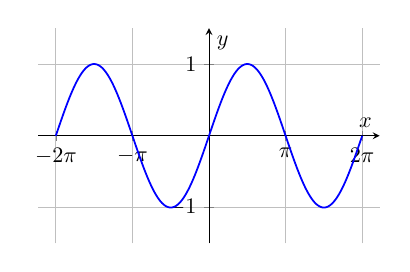
\begin{tikzpicture}[scale=0.8]
        \begin{axis}[
          axis lines = center,
          xlabel = $x$,
          ylabel = $y$,
          domain = -2*pi:2*pi,
          samples = 200,
          grid = major,
          xmin = -7, xmax = 7,
          ymin = -1.5, ymax = 1.5,
          xtick = {-6.28, -3.14, 0, 3.14, 6.28},
          xticklabels = {$-2\pi$, $-\pi$, $0$, $\pi$, $2\pi$},
          ytick = {-1, 0, 1},
          width = 7cm,
          height = 5cm
        ]
        \addplot[blue, thick] {sin(deg(x))};
        \end{axis}
      \end{tikzpicture}
      \caption{$\phi_1$}
    \end{subfigure}
    \hfill 
    \begin{subfigure}[b]{0.48\textwidth}
      \centering
      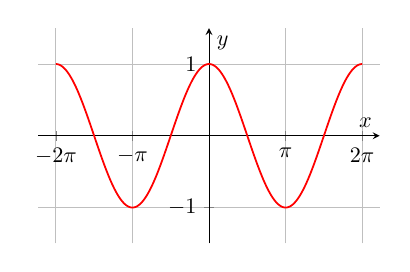
\begin{tikzpicture}[scale=0.8]
        \begin{axis}[
          axis lines = center,
          xlabel = $x$,
          ylabel = $y$,
          domain = -2*pi:2*pi,
          samples = 200,
          grid = major,
          xmin = -7, xmax = 7,
          ymin = -1.5, ymax = 1.5,
          xtick = {-6.28, -3.14, 0, 3.14, 6.28},
          xticklabels = {$-2\pi$, $-\pi$, $0$, $\pi$, $2\pi$},
          ytick = {-1, 0, 1},
          width = 7cm,
          height = 5cm
        ]
        \addplot[red, thick] {cos(deg(x))};
        \end{axis}
      \end{tikzpicture}
      \caption{$\phi_2$}
    \end{subfigure}
    
    \begin{subfigure}[b]{0.48\textwidth}
      \centering
      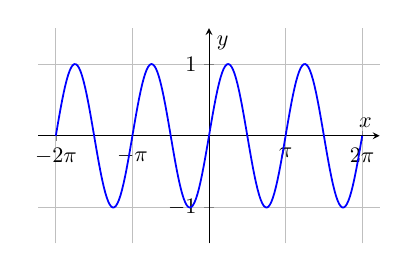
\begin{tikzpicture}[scale=0.8]
        \begin{axis}[
          axis lines = center,
          xlabel = $x$,
          ylabel = $y$,
          domain = -2*pi:2*pi,
          samples = 200,
          grid = major,
          xmin = -7, xmax = 7,
          ymin = -1.5, ymax = 1.5,
          xtick = {-6.28, -3.14, 0, 3.14, 6.28},
          xticklabels = {$-2\pi$, $-\pi$, $0$, $\pi$, $2\pi$},
          ytick = {-1, 0, 1},
          width = 7cm,
          height = 5cm
        ]
        \addplot[blue, thick] {sin(deg(2*x))};
        \end{axis}
      \end{tikzpicture}
      \caption{$\phi_3$}
    \end{subfigure}
    \hfill 
    \begin{subfigure}[b]{0.48\textwidth}
      \centering
      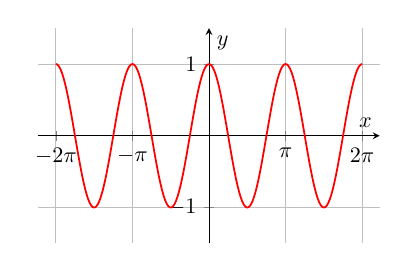
\begin{tikzpicture}[scale=0.8]
        \begin{axis}[
          axis lines = center,
          xlabel = $x$,
          ylabel = $y$,
          domain = -2*pi:2*pi,
          samples = 200,
          grid = major,
          xmin = -7, xmax = 7,
          ymin = -1.5, ymax = 1.5,
          xtick = {-6.28, -3.14, 0, 3.14, 6.28},
          xticklabels = {$-2\pi$, $-\pi$, $0$, $\pi$, $2\pi$},
          ytick = {-1, 0, 1},
          width = 7cm,
          height = 5cm
        ]
        \addplot[red, thick] {cos(deg(2*x))};
        \end{axis}
      \end{tikzpicture}
      \caption{$\phi_4$}
    \end{subfigure}
    \caption{The fourier basis as the eigenbases.}
  \end{figure}

  Now, we can fix the first term in the kernel and it will be function of the second term $K_x (\cdot) = K(x, \cdot)$. We do this for all $x \in \mathbb{R}$, which form the basis of our RKHS, and it consists of all functions that are finite linear combinations of these $K_x$'s. This creates a vector space, and we can add a well-defined inner product. Finally, this inner product induces a norm which can be used to complete this inner product space into a Hilbert space. 

  \begin{definition}[Reproducing Kernel Hilbert Space]
    Given a kernel $K$, the \textbf{reproducing kernel Hilbert space (RKHS)} is defined as the completion of the vector space consisting of functions $f: \mathcal{X} \to \mathbb{R}$ of the form
    \begin{equation}
      f = \sum_{i=1}^n \alpha_i K_{x_i} (x) 
    \end{equation}
    for all number of combinations $n \in \mathbb{N}$,\footnote{Note it must be finite.} for all choices of centers $x_1, \ldots, x_n \in \mathcal{X}$, and for all coefficients $\alpha_1, \ldots, \alpha_n \in \mathbb{R}$. The completion\footnote{The completion allows us to define for countable sums as well by taking limits.} is with respect to the inner product 
    \begin{equation}
      \langle f, g \rangle_{\mathcal{H}} = \sum_{i=1}^n \sum_{j=1}^m \alpha_i \beta_j K(x_i, x_j)
    \end{equation}
  \end{definition}
  \begin{proof}
    We know that a completion of a vector space is a vector space. So it remains to show that $\langle \cdot, \cdot \rangle_{\mathcal{H}}$ is a well-defined inner product. It follows from the positive semidefiniteness and symmetry of $K$ that $\langle f, f \rangle \geq 0$ with $\langle f, f \rangle = 0 \iff f = 0$ and $\langle f, g \rangle = \langle g, f \rangle$. Bilinearity is also easy to prove. 
  \end{proof}

  It turns out that the norm of an RKHS tends to be a measure of the smoothness, which isn't obvious at first. Wigglier functions tend to have bigger norms. 

  Another nice property is that since $K_x$ is itself in the RKHS, we can take the inner product of $f$ and $K_x$, which just gives us back the evaluation of $f$ at $x$. 

  \begin{theorem}[Reproducing Property of RKHS]
    An RKHS satisfies the \textbf{reproducing property}, which means that taking the inner product of a function $f$ and a kernel $K_x$ gives you the evaluation of $f$ at $x$. 
    \begin{equation}
      \langle f, K_x \rangle_{\mathcal{H}} = f(x)
    \end{equation}
    and therefore it also means that $\langle K_x, K_x \rangle_{\mathcal{H}} = K(x, x)$. This also means that $K_x$ is the evaluation functional in the dual space of $\mathcal{H}$ and this evaluation functional $\delta_x$ is continuous, which is not generally true in $L^p$ spaces. 
  \end{theorem}
  \begin{proof}
    We can evaluate from the inner product 
    \begin{equation}
      f = \sum_i \alpha_i K_{x_i} \implies \langle f, K_x \rangle_K = \sum_i \alpha_i \langle K_{x_i}, K_x \rangle_K = \sum_i \alpha_i K(x_i, x) = f(x)
    \end{equation}
  \end{proof}

  This reproducing property tends to be very useful, especially in the corollary below. 

  \begin{corollary}[Convergence in RKHS]
    Convergence in norm implies pointwise convergence in RKHS. 
  \end{corollary}
  \begin{proof}
    Given that $f_n \rightarrow f$ in norm, we have that $||f_n - f|| \rightarrow 0$. Then for all points $x \in \mathcal{X}$, by Cauchy Schwartz we have 
    \begin{equation}
      |f_n(x) - f(x)| = |\langle f_n - f, K_x \rangle_{\mathcal{H}}| \leq ||f_n - f|| \cdot ||K_x|| \rightarrow 0
    \end{equation}
    An alternative method is to take the evaluation functional $\delta_x f = f(x)$. Then, for a sequence $f_n \to f$ in norm
    \begin{equation}
      \delta_x f_n = \langle f_n, K_x \rangle \to \langle f, f_x \rangle = f(x) = \delta_x f
    \end{equation}
    and so $f_n \to f$ implies $\delta_x f_x \to \delta_x f$. 
  \end{proof}

  \begin{theorem}[Moore-Aronszajn] 
    Any positive definite function $K$ is a reproducing kernel for some RKHS.  
  \end{theorem} 
  \begin{proof} 
    We won't be too rigorous about this since this is not a functional analysis course. Assume that we have a positive definite kernel $K: X \times X \rightarrow \mathbb{R}$, where $X$ is some measurable set, and we will show how to make a RKHS $\mathcal{H}_k$ such that $K$ is the reproducing kernel on $\mathcal{H}$. It turns out that $\mathcal{H}_k$ is unique up to isomorphism. Since $X$ exists, let us first define the set $S = \{ k_x \mid x \in X\}$ such that $k_x (y) \coloneqq K(x, y)$. Now let us define the vector space $V$ to be the span of $S$. Therefore, each element $v \in V$ can be written as 
    \[v = \sum_i \alpha_i k_{x_i}\]
    Now we want to define an inner product on $V$. By expanding out the vectors w.r.t. the basis and the properties of bilinearity, we have 
    \[\langle k_x, k_y \rangle_{V} = \bigg\langle \sum_i \alpha_i k_{x_i} , \sum_i \beta_i k_{y_i} \bigg\rangle = \sum_{i, j} \alpha_i \beta_j K(x_i, y_j)\] 
    At this point, $V$ is not necessarily complete, but we can force it to be complete by taking the limits of all Cauchy sequences and adding them to $V$. In order to complete the construction, we need to ensure that $K$ is continuous and doesn't diverge, i.e. 
    \[\iint K^2 (x, y) \,dx\,dy < +\infty\]
    which is a property known as finite trace.\footnote{Too much to write down here at this point, but for further information look at $\href{http://users.umiacs.umd.edu/~hal/docs/daume04rkhs.pdf}{the article here}$.}
  \end{proof}

  Now at first glance, this abstract construction makes it hard to determine what kind of functions there are in a RKHS generated by some kernel. Conversely, given some RKHS, it's not always easy to know which kernel it came from. 

  \begin{example}[Fourier Basis]
    Let us take the vector space of all real functions $f$ for which its Fourier transform is supported on some finite interval $[-a, a]$. This is a RKHS with the kernel function 
    \begin{equation}
      K(x, y) = \frac{\sin(a(y - x))}{a(y - x)}
    \end{equation}
    with the inner product $\langle f, g \rangle = \int f(x) g(x) \,dx$.
  \end{example}

  \begin{example}[Some Sobelov Spaces are RKHS]
    Let us take the Sobelov space $W_{1, 2}$ of all functions $f: [0, 1] \rightarrow \mathbb{R}$ satisfying 
    \begin{equation}
      \int (f^\prime (x))^2 \,dx < \infty
    \end{equation} 
    This is a RKHS with the kernel function 
    \begin{equation}
      K(x, y) = \begin{cases} 1 + xy + \frac{xy^2}{2} - \frac{y^3}{6} & \text{ if } 0 \leq y \leq x \leq 1 \\
        1 + xy + \frac{x^2 y}{2} - \frac{x^3}{6} & \text{ if } 0 \leq x \leq y \leq 1 \end{cases}
    \end{equation}
  \end{example}

  The last two examples should show you that it's not easy to know what the elements of a RKHS look like for a given kernel. Let's try to build some intuition for this. A consequence of Mercer's theorem is that it gives us a conceptually easier way to think of functions $f$. We can either think of it in the finite kernel expansion---as defined in the RKHS---or as an infinite linear combination of its orthonormal eigenbasis. 
  \begin{equation}
    f(x) = \sum_{i=1}^n \alpha_i K_{x_i} (x), \qquad f(x) = \sum_{j=1}^\infty \lambda_j \phi_j(x)
  \end{equation}
  Conceptually, the basis expansion is nicer since it appeals to traditional linear algebra in that vectors are a linear combination of basis vectors. But when doing computation, the finite sum of the kernel expansion is nicer. In fact, when you talk about feature maps (e.g. in support vector machines), you're really just creating the map from $x \in \mathcal{X}$ into the infinite dimensional vector space 
  \begin{equation}
    x \mapsto \Phi(x) = \big( \sqrt{\lambda_1} \phi_1(x), \sqrt{\lambda_2} \phi_2(x), \ldots \big)
  \end{equation}
  Therefore, you can either just work with $x$ in the RKHS or work with the features $\Phi$ in a higher dimensional Euclidean space. The inner product between two functions is equal to the inner product between their feature maps. 
  \begin{equation}
    \langle f, g \rangle = \sum_i \frac{\alpha_i \beta_i}{\lambda_i} 
  \end{equation}
  With this eigenbasis expansion, $f, g$ must satisfy some smoothness constraints, and since the $\lambda_i$'s are getting smaller, the $\alpha_i$ and $\beta_i$ must die off quickly, making the sum finite. But we're never going to be actually computing this way since it's much easier to compute with the kernel expansion. 

  \begin{theorem}[Representer Theorem]
    
  \end{theorem}

  Now later, when we get to kernel methods, we will see that the whole point of working in RKHS is that we know that the minimizer of the regularized loss has the form above by the representer theorem. 

  It turns out that even though we are working in an infinite-dimensional space, we only have to optimize over the observed data, and so this becomes an finite-dimensional optimization. 

